% File nhập kho đợt 24: Cụm 16 (Đề 2 & Đề 3 - Đề 47 & 48) - ĐỢT CUỐI CÙNG
% Nguồn: Bộ Đề tham khảo Tuyển sinh 10 năm học 2026-2027 của Sở GD&ĐT TP.HCM

% ==============================================================================
% CỤM 16 - ĐỀ 2 (ĐỀ SỐ 47)
% ==============================================================================

\begin{bt}%[9D6H18-2]
% nguon: Đề tham khảo Tuyển sinh 10 năm học 2026-2027 Sở GD&ĐT TP.HCM - Cụm 16 - Đề 2 - Bài 1
Cho hàm số $y = \dfrac{1}{3}x^2$ có đồ thị là parabol $(P)$.
\begin{enumerate}[a)]
	\item Vẽ đồ thị $(P)$ trên hệ trục tọa độ.
	\item Tìm tọa độ các điểm thuộc $(P)$ có hoành độ là nghiệm của phương trình $x^2 + 3x - 18 = 0$.
\end{enumerate}
\loigiai{
\begin{enumerate}[a)]
	\item Bảng giá trị tương ứng của $x$ và $y$:
	\begin{center}
		\begin{tabular}{|c|c|c|c|c|c|}
			\hline
			$x$ & $-6$ & $-3$ & $0$ & $3$ & $6$ \\ \hline
			$y = \dfrac{1}{3}x^2$ & $12$ & $3$ & $0$ & $3$ & $12$ \\ \hline
		\end{tabular}
	\end{center}
	Đồ thị $(P)$ là một đường parabol đi qua các điểm $(-6; 12)$, $(-3; 3)$, $(0; 0)$, $(3; 3)$, $(6; 12)$, có đỉnh là gốc tọa độ $O(0; 0)$ và nhận trục tung làm trục đối xứng.
	\begin{center}
		\begin{tikzpicture}[>=stealth, scale=0.6]
			\draw[->] (-7,0) -- (7,0) node[below] {$x$};
			\draw[->] (0,-1) -- (0,13) node[left] {$y$};
			\draw (0,0) node[below left] {$O$};
			\foreach \x in {-6,-3,3,6}
				\draw (\x,0.1) -- (\x,-0.1) node[below] {$\x$};
			\foreach \y in {3,12}
				\draw (0.1,\y) -- (-0.1,\y) node[left] {$\y$};
			\draw[dashed] (-6,0) -- (-6,12) -- (6,12) -- (6,0);
			\draw[dashed] (-3,0) -- (-3,3) -- (3,3) -- (3,0);
			\draw[smooth,samples=100,domain=-6.2:6.2,thick,blue] plot(\x,{1/3*(\x)^2});
			\node[blue,right] at (5,8.3) {$(P)\colon y=\frac{1}{3}x^2$};
			\fill (-6,12) circle (2pt) (-3,3) circle (2pt) (0,0) circle (2pt) (3,3) circle (2pt) (6,12) circle (2pt);
		\end{tikzpicture}
	\end{center}
	\item Phương trình $x^2 + 3x - 18 = 0$.\\
	Ta có $\Delta = 3^2 - 4 \cdot 1 \cdot (-18) = 9 + 72 = 81 > 0$.\\
	Phương trình có hai nghiệm phân biệt:
	$$x_1 = \dfrac{-3 + \sqrt{81}}{2} = 3;\quad x_2 = \dfrac{-3 - \sqrt{81}}{2} = -6.$$
	Với $x_1 = 3 \implies y_1 = \dfrac{1}{3} \cdot 3^2 = 3$, ta được điểm $A(3; 3)$.\\
	Với $x_2 = -6 \implies y_2 = \dfrac{1}{3} \cdot (-6)^2 = 12$, ta được điểm $B(-6; 12)$.\\
	Vậy tọa độ các điểm cần tìm là $(3; 3)$ và $(-6; 12)$.
\end{enumerate}
}
\end{bt}

\begin{bt}%[9D6H20-2]
% nguon: Đề tham khảo Tuyển sinh 10 năm học 2026-2027 Sở GD&ĐT TP.HCM - Cụm 16 - Đề 2 - Bài 2
Cho phương trình $x^2 - x - 7 = 0$.
\begin{enumerate}[a)]
	\item Chứng minh rằng phương trình có hai nghiệm phân biệt $x_1$ và $x_2$.
	\item Không giải phương trình, hãy tính giá trị của biểu thức $P = x_1(x_1 - x_2) + x_2^2 + 2012$.
\end{enumerate}
\loigiai{
\begin{enumerate}[a)]
	\item Phương trình $x^2 - x - 7 = 0$ có các hệ số $a = 1$, $b = -1$, $c = -7$.\\
	Ta có $\Delta = b^2 - 4ac = (-1)^2 - 4 \cdot 1 \cdot (-7) = 1 + 28 = 29 > 0$.\\
	Vì $\Delta > 0$ nên phương trình luôn có hai nghiệm phân biệt $x_1, x_2$.
	\item Theo định lí Vi-ét, ta có:
	$$\begin{cases}
		x_1 + x_2 = -\dfrac{b}{a} = 1 \\
		x_1 x_2 = \dfrac{c}{a} = -7
	\end{cases}$$
	Ta biến đổi biểu thức $P$:
	\begin{align*}
		P &= x_1(x_1 - x_2) + x_2^2 + 2012 \\
		&= x_1^2 - x_1 x_2 + x_2^2 + 2012 \\
		&= (x_1^2 + x_2^2) - x_1 x_2 + 2012 \\
		&= \left[(x_1 + x_2)^2 - 2x_1 x_2\right] - x_1 x_2 + 2012 \\
		&= (x_1 + x_2)^2 - 3x_1 x_2 + 2012.
	\end{align*}
	Thay $x_1 + x_2 = 1$ và $x_1 x_2 = -7$ vào biểu thức $P$, ta được:
	$$P = 1^2 - 3 \cdot (-7) + 2012 = 1 + 21 + 2012 = 2034.$$
	Vậy $P = 2034$.
\end{enumerate}
}
\end{bt}

\begin{bt}%[9D8H26-3]
% nguon: Đề tham khảo Tuyển sinh 10 năm học 2026-2027 Sở GD&ĐT TP.HCM - Cụm 16 - Đề 2 - Bài 3
Một cửa hàng bán điện thoại tổ chức chương trình rút thăm trúng thưởng. Trong một thùng có $60$ phiếu, bao gồm $15$ phiếu giảm giá $200\,000$ đồng, $20$ phiếu giảm giá $100\,000$ đồng, còn lại là số phiếu không có giảm giá. Một khách hàng rút ngẫu nhiên $1$ phiếu. Tính xác suất để khách hàng đó:
\begin{enumerate}[a)]
	\item Nhận được bất kỳ phiếu giảm giá nào.
	\item Không nhận được phiếu giảm giá.
\end{enumerate}
\loigiai{
Vì khách hàng rút ngẫu nhiên $1$ phiếu từ thùng có $60$ phiếu nên số kết quả có thể xảy ra là $n(\Omega) = 60$.
\begin{enumerate}[a)]
	\item Gọi $A$ là biến cố: ``Khách hàng nhận được bất kỳ phiếu giảm giá nào''.\\
	Số phiếu giảm giá có trong thùng là $15 + 20 = 35$ (phiếu).\\
	Do đó số kết quả thuận lợi cho biến cố $A$ là $n(A) = 35$.\\
	Xác suất để khách hàng nhận được bất kỳ phiếu giảm giá nào là:
	$$P(A) = \dfrac{n(A)}{n(\Omega)} = \dfrac{35}{60} = \dfrac{7}{12}.$$
	\item Gọi $B$ là biến cố: ``Khách hàng không nhận được phiếu giảm giá''.\\
	Số phiếu không có giảm giá trong thùng là $60 - 35 = 25$ (phiếu).\\
	Do đó số kết quả thuận lợi cho biến cố $B$ là $n(B) = 25$.\\
	Xác suất để khách hàng không nhận được phiếu giảm giá là:
	$$P(B) = \dfrac{n(B)}{n(\Omega)} = \dfrac{25}{60} = \dfrac{5}{12}.$$
\end{enumerate}
}
\end{bt}

\begin{bt}%[9H0V31-3]
% nguon: Đề tham khảo Tuyển sinh 10 năm học 2026-2027 Sở GD&ĐT TP.HCM - Cụm 16 - Đề 2 - Bài 4
Một lon sơn dầu có dạng hình trụ có chiều cao $h = 12\text{ cm}$ và đường kính đường tròn mặt đáy là $2x\text{ cm}$.
\begin{enumerate}[a)]
	\item Viết biểu thức theo $x$ biểu diễn thể tích $V\text{ (cm}^3\text{)}$ của lon sơn dầu.
	\item Biết $x = 5{,}5\text{ cm}$. Bác An muốn sơn một cánh cổng làm bằng sắt hình chữ nhật có chiều cao là $2{,}5\text{ m}$ và chiều rộng là $3\text{ m}$. Hỏi bác An cần mua ít nhất bao nhiêu lon sơn loại như trên để sơn phủ cả hai mặt của cánh cổng, biết mỗi lon sơn phủ được nhiều nhất là $3{,}5\text{ m}^2$?
\end{enumerate}
\loigiai{
\begin{enumerate}[a)]
	\item Lon sơn có đáy là hình tròn đường kính $2x\text{ cm}$ nên bán kính đáy là $R = \dfrac{2x}{2} = x\text{ (cm)}$.\\
	Thể tích của lon sơn hình trụ là:
	$$V = \pi R^2 h = \pi \cdot x^2 \cdot 12 = 12\pi x^2\text{ (cm}^3\text{)}.$$
	Vậy biểu thức biểu diễn thể tích là $V = 12\pi x^2\text{ (cm}^3\text{)}$.
	\item Diện tích một mặt của cánh cổng hình chữ nhật là:
	$$2{,}5 \cdot 3 = 7{,}5\text{ (m}^2\text{)}.$$
	Vì sơn phủ cả hai mặt của cánh cổng nên tổng diện tích cần sơn là:
	$$S = 7{,}5 \cdot 2 = 15\text{ (m}^2\text{)}.$$
	Số lon sơn cần dùng ít nhất là:
	$$\dfrac{15}{3{,}5} = \dfrac{30}{7} \approx 4{,}28\text{ (lon)}.$$
	Vì số lon sơn phải mua là số tự nhiên nên bác An cần mua ít nhất $5$ lon sơn loại trên.
\end{enumerate}
}
\end{bt}

\begin{bt}%[9D6V21-3]
% nguon: Đề tham khảo Tuyển sinh 10 năm học 2026-2027 Sở GD&ĐT TP.HCM - Cụm 16 - Đề 2 - Bài 5
Một khu hồ bơi gồm ba phần: Hồ chính có dạng hình chữ nhật với kích thước ngoài là $50\text{ m} \times 20\text{ m}$; một hồ bán nguyệt lớn gắn liền với hồ chính có đường kính ngoài $30\text{ m}$; một hồ bán nguyệt nhỏ gắn liền với hồ chính có đường kính ngoài $20\text{ m}$. Bề mặt thành hồ ở tất cả các phần đều rộng $0{,}3\text{ m}$. Chiều sâu của các hồ như sau: Hồ chính sâu $2\text{ m}$; hồ bán nguyệt lớn sâu $1{,}2\text{ m}$; hồ bán nguyệt nhỏ sâu $0{,}8\text{ m}$.
\begin{enumerate}[a)]
	\item Tính tổng diện tích bề mặt thành hồ của toàn bộ khu hồ bơi (kết quả làm tròn đến hai chữ số thập phân).
	\item Sau khi xây dựng xong, khu hồ bơi được bơm nước: Hồ chính được bơm đầy nước; hai hồ bán nguyệt chỉ bơm đến $\dfrac{3}{4}$ độ sâu thiết kế. Hệ thống bơm có lưu lượng $400\text{ m}^3\text{/giờ}$ và hoạt động liên tục trong $6\text{ giờ}$. Hỏi toàn bộ khu hồ bơi có được bơm đủ nước theo đúng quy trình hay không?
\end{enumerate}
\loigiai{
\begin{enumerate}[a)]
	\item Diện tích bề mặt thành hồ chính (hình chữ nhật) là:
	$$S_1 = 50 \cdot 20 - (50 - 2 \cdot 0{,}3)(20 - 2 \cdot 0{,}3) = 1000 - 49{,}4 \cdot 19{,}4 = 41{,}64\text{ (m}^2\text{)}.$$
	Bán kính ngoài của hồ bán nguyệt lớn là $R_1 = 30 : 2 = 15\text{ (m)}$, bán kính trong là $r_1 = 15 - 0{,}3 = 14{,}7\text{ (m)}$.\\
	Diện tích bề mặt thành hồ bán nguyệt lớn (chỉ tính phần viền cong ngoài) là:
	$$S_2 = \dfrac{1}{2}\pi (R_1^2 - r_1^2) = \dfrac{1}{2}\pi (15^2 - 14{,}7^2) = 4{,}455\pi\text{ (m}^2\text{)}.$$
	Bán kính ngoài của hồ bán nguyệt nhỏ là $R_2 = 20 : 2 = 10\text{ (m)}$, bán kính trong là $r_2 = 10 - 0{,}3 = 9{,}7\text{ (m)}$.\\
	Diện tích bề mặt thành hồ bán nguyệt nhỏ (chỉ tính phần viền cong ngoài) là:
	$$S_3 = \dfrac{1}{2}\pi (R_2^2 - r_2^2) = \dfrac{1}{2}\pi (10^2 - 9{,}7^2) = 2{,}955\pi\text{ (m}^2\text{)}.$$
	Tổng diện tích bề mặt thành hồ của toàn bộ khu hồ bơi là:
	$$S = S_1 + S_2 + S_3 = 41{,}64 + 4{,}455\pi + 2{,}955\pi = 41{,}64 + 7{,}41\pi \approx 64{,}92\text{ (m}^2\text{)}.$$
	\item Kích thước lòng trong hồ chính là $49{,}4\text{ m} \times 19{,}4\text{ m}$ và sâu $2\text{ m}$.\\
	Thể tích nước bơm đầy hồ chính là:
	$$V_1 = 49{,}4 \cdot 19{,}4 \cdot 2 = 1916{,}72\text{ (m}^3\text{)}.$$
	Thể tích nước bơm vào hồ bán nguyệt lớn ($\dfrac{3}{4}$ độ sâu) là:
	$$V_2 = \dfrac{1}{2}\pi \cdot (14{,}7)^2 \cdot \left(1{,}2 \cdot \dfrac{3}{4}\right) = \dfrac{1}{2}\pi \cdot 216{,}09 \cdot 0{,}9 = 97{,}2405\pi\text{ (m}^3\text{)}.$$
	Thể tích nước bơm vào hồ bán nguyệt nhỏ ($\dfrac{3}{4}$ độ sâu) là:
	$$V_3 = \dfrac{1}{2}\pi \cdot (9{,}7)^2 \cdot \left(0{,}8 \cdot \dfrac{3}{4}\right) = \dfrac{1}{2}\pi \cdot 94{,}09 \cdot 0{,}6 = 28{,}227\pi\text{ (m}^3\text{)}.$$
	Tổng thể tích nước cần bơm vào toàn bộ khu hồ bơi là:
	$$V = V_1 + V_2 + V_3 = 1916{,}72 + 97{,}2405\pi + 28{,}227\pi = 1916{,}72 + 125{,}4675\pi \approx 2310{,}89\text{ (m}^3\text{)}.$$
	Tổng lượng nước hệ thống bơm cung cấp được trong $6\text{ giờ}$ là:
	$$V_{\text{bơm}} = 400 \cdot 6 = 2400\text{ (m}^3\text{)}.$$
	Vì $2400 > 2310{,}89$ nên toàn bộ khu hồ bơi được bơm đủ nước theo đúng quy trình.
\end{enumerate}
}
\end{bt}

\begin{bt}%[9D1H3-4]
% nguon: Đề tham khảo Tuyển sinh 10 năm học 2026-2027 Sở GD&ĐT TP.HCM - Cụm 16 - Đề 2 - Bài 6
Liên đội một trường THCS đã phát động phong trào kế hoạch nhỏ hai lần trong một năm học. Đợt thứ nhất chi đội lớp 9A và chi đội lớp 9B thu gom được tổng cộng $45\text{ kg}$ giấy vụn. Trong đợt thứ hai, chi đội lớp 9A gom vượt mức $25\%$ và chi đội lớp 9B gom vượt mức $30\%$ so với đợt đầu, do đó tổng số giấy cả hai chi đội gom được nhiều hơn đợt đầu là $12{,}5\text{ kg}$. Hỏi mỗi chi đội đã gom được bao nhiêu kilôgam giấy vụn trong đợt đầu?
\loigiai{
Gọi số giấy vụn chi đội lớp 9A và chi đội lớp 9B thu gom được trong đợt đầu lần lượt là $x$ và $y$ (đơn vị: $\text{kg}$, điều kiện $0 < x, y < 45$).\\
Đợt đầu cả hai chi đội thu gom được tổng cộng $45\text{ kg}$ giấy vụn, nên ta có phương trình:
$$x + y = 45. \quad (1)$$
Trong đợt thứ hai:
\begin{itemize}
	\item Chi đội lớp 9A gom vượt mức $25\%$, tức là vượt thêm $25\%x = 0{,}25x\text{ (kg)}$.
	\item Chi đội lớp 9B gom vượt mức $30\%$, tức là vượt thêm $30\%y = 0{,}3y\text{ (kg)}$.
\end{itemize}
Tổng số giấy vượt thêm của cả hai chi đội là $12{,}5\text{ kg}$, nên ta có phương trình:
$$0{,}25x + 0{,}3y = 12{,}5. \quad (2)$$
Từ (1) và (2) ta có hệ phương trình:
$$\begin{cases}
	x + y = 45 \\
	0{,}25x + 0{,}3y = 12{,}5
\end{cases}
\iff
\begin{cases}
	0{,}25x + 0{,}25y = 11{,}25 \\
	0{,}25x + 0{,}3y = 12{,}5
\end{cases}
\iff
\begin{cases}
	0{,}05y = 1{,}25 \\
	x = 45 - y
\end{cases}
\iff
\begin{cases}
	y = 25 \\
	x = 20
\end{cases}\text{ (thỏa mãn điều kiện).}$$
Vậy trong đợt đầu, chi đội lớp 9A gom được $20\text{ kg}$ giấy vụn và chi đội lớp 9B gom được $25\text{ kg}$ giấy vụn.
}
\end{bt}

\begin{bt}%[9H9C29-3]
% nguon: Đề tham khảo Tuyển sinh 10 năm học 2026-2027 Sở GD&ĐT TP.HCM - Cụm 16 - Đề 2 - Bài 7
Cho nửa đường tròn $(O; R)$ có đường kính $AB$. Cùng phía với nửa đường tròn, vẽ lần lượt các tia tiếp tuyến $Ax, By$ với $(O; R)$ tại $A$ và $B$. Gọi $I$ là trung điểm của đoạn thẳng $AO$. Lấy hai điểm $C \in Ax$ và $D \in By$ sao cho $\widehat{CID} = 90^\circ$. Gọi $H$ là hình chiếu vuông góc của $I$ lên $CD$.
\begin{enumerate}[a)]
	\item Chứng minh tứ giác $ACHI$ nội tiếp và $\widehat{AHB} = 90^\circ$.
	\item Gọi $E$ là giao điểm của $AH$ và $IC$, $F$ là giao điểm của $BH$ và $ID$. Chứng minh $EF \parallel AB$ và tích $AC \cdot BD$ không đổi.
	\item Xác định vị trí các điểm $C$ trên $Ax$ và $D$ trên $By$ để diện tích tam giác $CID$ đạt giá trị nhỏ nhất.
\end{enumerate}
\loigiai{
\begin{center}
	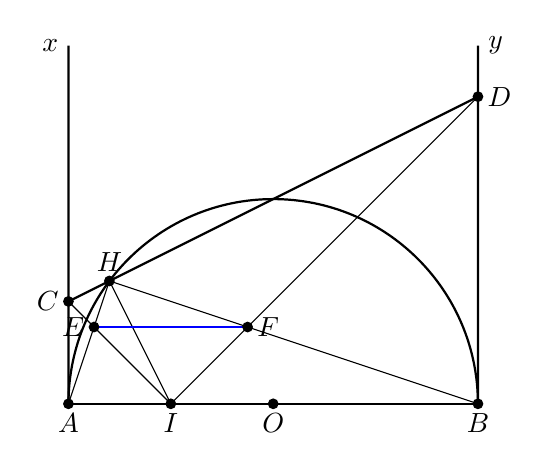
\begin{tikzpicture}[>=stealth, scale=1.3]
		\coordinate (O) at (0,0);
		\coordinate (A) at (-2,0);
		\coordinate (B) at (2,0);
		\coordinate (I) at (-1,0);
		\draw[thick] (2,0) arc (0:180:2);
		\draw[thick] (A) -- (B);
		\coordinate (C) at (-2,1);
		\coordinate (D) at (2,3);
		\coordinate (H) at (-1.6,1.2);
		\coordinate (E) at (-1.75,0.75);
		\coordinate (F) at (-0.25,0.75);
		\draw[thick] (A) -- (-2,3.5) node[left] {$x$};
		\draw[thick] (B) -- (2,3.5) node[right] {$y$};
		\draw[thick] (C) -- (D);
		\draw (I) -- (C) (I) -- (D) (I) -- (H);
		\draw (A) -- (H) -- (B);
		\draw[thick, blue] (E) -- (F);
		\fill (O) circle (1.5pt) node[below] {$O$};
		\fill (A) circle (1.5pt) node[below] {$A$};
		\fill (B) circle (1.5pt) node[below] {$B$};
		\fill (I) circle (1.5pt) node[below] {$I$};
		\fill (C) circle (1.5pt) node[left] {$C$};
		\fill (D) circle (1.5pt) node[right] {$D$};
		\fill (H) circle (1.5pt) node[above] {$H$};
		\fill (E) circle (1.5pt) node[left] {$E$};
		\fill (F) circle (1.5pt) node[right] {$F$};
	\end{tikzpicture}
\end{center}
\begin{enumerate}[a)]
	\item Ta có $Ax$ là tiếp tuyến của $(O)$ tại $A$ nên $Ax \perp AB \implies \widehat{CAI} = 90^\circ$.\\
	Vì $H$ là hình chiếu của $I$ lên $CD$ nên $IH \perp CD \implies \widehat{CHI} = 90^\circ$.\\
	Hai đỉnh $A$ và $H$ kề nhau cùng nhìn đoạn $CI$ dưới góc $90^\circ$, suy ra tứ giác $ACHI$ nội tiếp đường tròn đường kính $CI$.\\
	Chứng minh tương tự: Vì $By \perp AB$ nên $\widehat{DBI} = 90^\circ$; và $\widehat{DHI} = 90^\circ$, do đó tứ giác $BDIH$ nội tiếp đường tròn đường kính $DI$.\\
	Từ tứ giác $ACHI$ nội tiếp, ta có $\widehat{AHI} = \widehat{ACI}$ (hai góc nội tiếp cùng chắn cung $AI$).\\
	Từ tứ giác $BDIH$ nội tiếp, ta có $\widehat{IHB} = \widehat{IDB}$ (hai góc nội tiếp cùng chắn cung $IB$).\\
	Do đó:
	$$\widehat{AHB} = \widehat{AHI} + \widehat{IHB} = \widehat{ACI} + \widehat{IDB}.$$
	Mặt khác, trong tam giác $CAI$ vuông tại $A$, ta có $\widehat{ACI} + \widehat{AIC} = 90^\circ$.\\
	Lại có $\widehat{AIC} + \widehat{CID} + \widehat{DIB} = 180^\circ \implies \widehat{AIC} + \widehat{DIB} = 180^\circ - 90^\circ = 90^\circ$.\\
	Suy ra $\widehat{ACI} = \widehat{DIB}$ (cùng phụ với $\widehat{AIC}$).\\
	Trong tam giác $DBI$ vuông tại $B$, ta có $\widehat{DIB} + \widehat{IDB} = 90^\circ \implies \widehat{ACI} + \widehat{IDB} = 90^\circ$.\\
	Vậy $\widehat{AHB} = 90^\circ$.
	\item Tam giác $EHF$ có $\widehat{EHF} = \widehat{AHB} = 90^\circ$, tam giác $EIF$ có $\widehat{EIF} = \widehat{CID} = 90^\circ$.\\
	Do đó hai điểm $H$ và $I$ cùng nhìn đoạn $EF$ dưới góc vuông, suy ra tứ giác $IEHF$ nội tiếp đường tròn đường kính $EF$.\\
	Suy ra $\widehat{IEF} = \widehat{IHF}$ (hai góc nội tiếp cùng chắn cung $IF$).\\
	Mà $\widehat{IHF} = \widehat{IHB} = \widehat{IDB} = \widehat{AIC}$.\\
	Do đó $\widehat{IEF} = \widehat{AIC}$. Mà hai góc này ở vị trí so le trong nên $EF \parallel AB$.\\
	Xét $\triangle CAI$ và $\triangle IBD$ có:
	$$\widehat{CAI} = \widehat{IBD} = 90^\circ,\quad \widehat{ACI} = \widehat{DIB}\text{ (chứng minh trên)}.$$
	Suy ra $\triangle CAI \sim \triangle IBD$ (g.g), do đó:
	$$\dfrac{AC}{IB} = \dfrac{AI}{BD} \implies AC \cdot BD = AI \cdot IB.$$
	Vì $I$ là trung điểm của $AO$ nên $AI = \dfrac{R}{2}$, do đó:
	$$IB = AB - AI = 2R - \dfrac{R}{2} = \dfrac{3R}{2}.$$
	Suy ra:
	$$AC \cdot BD = \dfrac{R}{2} \cdot \dfrac{3R}{2} = \dfrac{3R^2}{4}.$$
	Vì $R$ không đổi nên tích $AC \cdot BD$ không đổi.
	\item Tam giác $CID$ vuông tại $I$ nên diện tích là:
	$$S_{\triangle CID} = \dfrac{1}{2} IC \cdot ID.$$
	Vì $\triangle CAI \sim \triangle IBD \implies \dfrac{IC}{ID} = \dfrac{AC}{IB} \implies ID = \dfrac{IB \cdot IC}{AC}$.\\
	Do đó:
	$$S_{\triangle CID} = \dfrac{1}{2} IC \cdot \dfrac{IB \cdot IC}{AC} = \dfrac{1}{2} \cdot \dfrac{IB}{AC} \cdot IC^2.$$
	Trong tam giác $CAI$ vuông tại $A$, ta có $IC^2 = AC^2 + AI^2$. Suy ra:
	$$S_{\triangle CID} = \dfrac{1}{2} \cdot \dfrac{IB}{AC} (AC^2 + AI^2) = \dfrac{1}{2} IB \left(AC + \dfrac{AI^2}{AC}\right).$$
	Áp dụng bất đẳng thức Cô-si cho hai số dương $AC$ và $\dfrac{AI^2}{AC}$:
	$$AC + \dfrac{AI^2}{AC} \ge 2\sqrt{AC \cdot \dfrac{AI^2}{AC}} = 2AI.$$
	Suy ra:
	$$S_{\triangle CID} \ge \dfrac{1}{2} IB \cdot 2AI = AI \cdot IB = \dfrac{3R^2}{4}.$$
	Dấu ``='' xảy ra khi và chỉ khi:
	$$AC = \dfrac{AI^2}{AC} \iff AC = AI = \dfrac{R}{2}.$$
	Khi đó $BD = \dfrac{3R^2}{4} : AC = \dfrac{3R^2}{4} : \dfrac{R}{2} = \dfrac{3R}{2}$.\\
	Vậy diện tích tam giác $CID$ đạt giá trị nhỏ nhất bằng $\dfrac{3R^2}{4}$ khi điểm $C$ thuộc tia $Ax$ sao cho $AC = \dfrac{R}{2}$ và điểm $D$ thuộc tia $By$ sao cho $BD = \dfrac{3R}{2}$.
\end{enumerate}
}
\end{bt}

% ==============================================================================
% CỤM 16 - ĐỀ 3 (ĐỀ SỐ 48) - ĐỀ CUỐI CÙNG CỦA TOÀN BỘ 16 CỤM!
% ==============================================================================

\begin{bt}%[9D6H18-2]
% nguon: Đề tham khảo Tuyển sinh 10 năm học 2026-2027 Sở GD&ĐT TP.HCM - Cụm 16 - Đề 3 - Bài 1
Cho parabol $(P)\colon y = -x^2$.
\begin{enumerate}[a)]
	\item Vẽ đồ thị $(P)$ trên hệ trục tọa độ.
	\item Tìm tọa độ các điểm $M$ thuộc $(P)$ (khác gốc tọa độ) có hoành độ gấp đôi tung độ.
\end{enumerate}
\loigiai{
\begin{enumerate}[a)]
	\item Bảng giá trị tương ứng của $x$ và $y$:
	\begin{center}
		\begin{tabular}{|c|c|c|c|c|c|}
			\hline
			$x$ & $-2$ & $-1$ & $0$ & $1$ & $2$ \\ \hline
			$y = -x^2$ & $-4$ & $-1$ & $0$ & $-1$ & $-4$ \\ \hline
		\end{tabular}
	\end{center}
	Đồ thị $(P)$ là một đường parabol đi qua các điểm $(-2; -4)$, $(-1; -1)$, $(0; 0)$, $(1; -1)$, $(2; -4)$, nhận gốc tọa độ $O(0; 0)$ làm đỉnh và nhận trục tung làm trục đối xứng.
	\begin{center}
		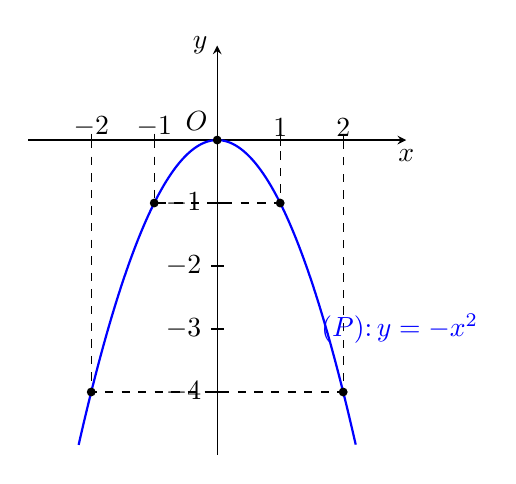
\begin{tikzpicture}[>=stealth, scale=0.8]
			\draw[->] (-3,0) -- (3,0) node[below] {$x$};
			\draw[->] (0,-5) -- (0,1.5) node[left] {$y$};
			\draw (0,0) node[above left] {$O$};
			\foreach \x in {-2,-1,1,2}
				\draw (\x,0.1) -- (\x,-0.1) node[above] {$\x$};
			\foreach \y in {-1,-2,-3,-4}
				\draw (0.1,\y) -- (-0.1,\y) node[left] {$\y$};
			\draw[dashed] (-2,0) -- (-2,-4) -- (2,-4) -- (2,0);
			\draw[dashed] (-1,0) -- (-1,-1) -- (1,-1) -- (1,0);
			\draw[smooth,samples=100,domain=-2.2:2.2,thick,blue] plot(\x,{-(\x)^2});
			\node[blue,right] at (1.5,-3) {$(P)\colon y=-x^2$};
			\fill (-2,-4) circle (2pt) (-1,-1) circle (2pt) (0,0) circle (2pt) (1,-1) circle (2pt) (2,-4) circle (2pt);
		\end{tikzpicture}
	\end{center}
	\item Điểm $M(x; y)$ thuộc $(P)$ nên $y = -x^2$.\\
	Vì hoành độ gấp đôi tung độ nên $x = 2y \implies y = \dfrac{1}{2}x$.\\
	Thay vào phương trình của $(P)$, ta được:
	$$\dfrac{1}{2}x = -x^2 \iff x^2 + \dfrac{1}{2}x = 0 \iff x\left(x + \dfrac{1}{2}\right) = 0 \iff \left[\begin{aligned} &x = 0 \\ &x = -\dfrac{1}{2}. \end{aligned}\right.$$
	Vì điểm $M$ khác gốc tọa độ nên $x \ne 0 \implies x = -\dfrac{1}{2}$.\\
	Khi đó $y = \dfrac{1}{2} \cdot \left(-\dfrac{1}{2}\right) = -\dfrac{1}{4}$.\\
	Vậy tọa độ điểm cần tìm là $M\left(-\dfrac{1}{2}; -\dfrac{1}{4}\right)$.
\end{enumerate}
}
\end{bt}

\begin{bt}%[9D6H20-2]
% nguon: Đề tham khảo Tuyển sinh 10 năm học 2026-2027 Sở GD&ĐT TP.HCM - Cụm 16 - Đề 3 - Bài 2
Cho phương trình $2x^2 - 3x - 5 = 0$.
\begin{enumerate}[a)]
	\item Chứng minh phương trình trên có hai nghiệm phân biệt $x_1, x_2$.
	\item Không giải phương trình, tính giá trị của biểu thức $A = x_1^2 + x_2^2 + 3x_1 x_2$.
\end{enumerate}
\loigiai{
\begin{enumerate}[a)]
	\item Phương trình $2x^2 - 3x - 5 = 0$ có các hệ số $a = 2$, $b = -3$, $c = -5$.\\
	Ta có $\Delta = b^2 - 4ac = (-3)^2 - 4 \cdot 2 \cdot (-5) = 9 + 40 = 49 > 0$.\\
	Vì $\Delta > 0$ nên phương trình có hai nghiệm phân biệt $x_1, x_2$.
	\item Theo định lí Vi-ét, ta có:
	$$\begin{cases}
		x_1 + x_2 = -\dfrac{b}{a} = \dfrac{3}{2} \\
		x_1 x_2 = \dfrac{c}{a} = -\dfrac{5}{2}
	\end{cases}$$
	Ta biến đổi biểu thức $A$:
	$$A = x_1^2 + x_2^2 + 3x_1 x_2 = (x_1 + x_2)^2 - 2x_1 x_2 + 3x_1 x_2 = (x_1 + x_2)^2 + x_1 x_2.$$
	Thay $x_1 + x_2 = \dfrac{3}{2}$ và $x_1 x_2 = -\dfrac{5}{2}$ vào biểu thức $A$, ta được:
	$$A = \left(\dfrac{3}{2}\right)^2 + \left(-\dfrac{5}{2}\right) = \dfrac{9}{4} - \dfrac{5}{2} = \dfrac{9 - 10}{4} = -\dfrac{1}{4}.$$
	Vậy $A = -\dfrac{1}{4}$.
\end{enumerate}
}
\end{bt}

\begin{bt}%[9D8H26-3]
% nguon: Đề tham khảo Tuyển sinh 10 năm học 2026-2027 Sở GD&ĐT TP.HCM - Cụm 16 - Đề 3 - Bài 3
Trong hộp đựng các quả bóng cùng chất liệu, cùng kích thước và cùng khối lượng được đánh số lần lượt từ $1$ đến $10$.
\begin{enumerate}[a)]
	\item Xác định không gian mẫu và số kết quả có thể xảy ra của phép thử lấy ngẫu nhiên một quả bóng.
	\item Tính xác suất của các biến cố sau:
	\begin{itemize}
		\item $A$: ``Lấy ngẫu nhiên một quả bóng mà số được ghi trên đó là số chẵn''.
		\item $B$: ``Lấy ngẫu nhiên một quả bóng mà số được ghi trên đó là số nguyên tố''.
	\end{itemize}
\end{enumerate}
\loigiai{
\begin{enumerate}[a)]
	\item Phép thử lấy ngẫu nhiên một quả bóng từ hộp có các quả bóng đánh số từ $1$ đến $10$.\\
	Không gian mẫu của phép thử là:
	$$\Omega = \{1; 2; 3; 4; 5; 6; 7; 8; 9; 10\}.$$
	Số kết quả có thể xảy ra là $n(\Omega) = 10$.
	\item Tính xác suất của các biến cố:
	\begin{itemize}
		\item Biến cố $A$: ``Số được ghi trên quả bóng là số chẵn''.\\
		Các kết quả thuận lợi cho biến cố $A$ là: $\{2; 4; 6; 8; 10\}$.\\
		Số kết quả thuận lợi là $n(A) = 5$.\\
		Xác suất của biến cố $A$ là:
		$$P(A) = \dfrac{n(A)}{n(\Omega)} = \dfrac{5}{10} = \dfrac{1}{2}.$$
		\item Biến cố $B$: ``Số được ghi trên quả bóng là số nguyên tố''.\\
		Các kết quả thuận lợi cho biến cố $B$ là: $\{2; 3; 5; 7\}$.\\
		Số kết quả thuận lợi là $n(B) = 4$.\\
		Xác suất của biến cố $B$ là:
		$$P(B) = \dfrac{n(B)}{n(\Omega)} = \dfrac{4}{10} = \dfrac{2}{5}.$$
	\end{itemize}
\end{enumerate}
}
\end{bt}

\begin{bt}%[9H4V12-3]
% nguon: Đề tham khảo Tuyển sinh 10 năm học 2026-2027 Sở GD&ĐT TP.HCM - Cụm 16 - Đề 3 - Bài 4
Hôm chủ nhật vừa rồi, hai bạn Lâm và Dương rủ nhau đi câu cá. Lâm chở Dương bằng xe đạp từ nhà Lâm tại vị trí $A$ đến một hồ cá tại vị trí $B$. Trên đường đi phải băng qua một con dốc có đỉnh dốc ở vị trí $C$. Biết góc lên dốc $\widehat{CAH} = 5^\circ$, góc xuống dốc $\widehat{CBH} = 9^\circ$ và độ cao con dốc $CH = x\text{ (m)}$ ($H$ là hình chiếu của $C$ lên đường ngang $AB$).
\begin{enumerate}[a)]
	\item Biểu diễn theo $x$ quãng đường $S$ mà hai bạn đi từ nhà Lâm đến hồ cá.
	\item Bạn Lâm đạp xe lên dốc với vận tốc $10\text{ km/h}$, đi $10\text{ phút}$ thì đến đỉnh dốc, và từ đó thả dốc với vận tốc $18\text{ km/h}$. Tính thời gian hai bạn đi từ nhà đến điểm câu cá (theo phút và giây).
\end{enumerate}
\loigiai{
\begin{center}
	\begin{tikzpicture}[>=stealth, scale=1.2]
		\coordinate (A) at (0,0);
		\coordinate (H) at (4,0);
		\coordinate (B) at (6,0);
		\coordinate (C) at (4,1.5);
		\draw[thick] (A) -- (C) node[midway, above left] {lên dốc} -- (B) node[midway, above right] {xuống dốc};
		\draw[dashed] (A) -- (H) -- (B);
		\draw[dashed] (C) -- (H) node[midway, right] {$x\text{ (m)}$};
		\draw (3.7,0) -- (3.7,0.3) -- (4,0.3);
		\draw (0.8,0) arc (0:20:0.8) node[midway, right] {$5^\circ$};
		\draw (5.3,0) arc (180:143:0.7) node[midway, left] {$9^\circ$};
		\fill (A) circle (1.5pt) node[below] {$A$};
		\fill (B) circle (1.5pt) node[below] {$B$};
		\fill (C) circle (1.5pt) node[above] {$C$};
		\fill (H) circle (1.5pt) node[below] {$H$};
	\end{tikzpicture}
\end{center}
\begin{enumerate}[a)]
	\item Trong tam giác vuông $AHC$ vuông tại $H$, ta có:
	$$\sin A = \dfrac{CH}{AC} \implies AC = \dfrac{CH}{\sin 5^\circ} = \dfrac{x}{\sin 5^\circ}\text{ (m)}.$$
	Trong tam giác vuông $BHC$ vuông tại $H$, ta có:
	$$\sin B = \dfrac{CH}{BC} \implies BC = \dfrac{CH}{\sin 9^\circ} = \dfrac{x}{\sin 9^\circ}\text{ (m)}.$$
	Quãng đường $S$ mà hai bạn đi từ nhà đến hồ cá là:
	$$S = AC + BC = \dfrac{x}{\sin 5^\circ} + \dfrac{x}{\sin 9^\circ}\text{ (m)}.$$
	\item Đổi $10\text{ phút} = \dfrac{10}{60}\text{ giờ} = \dfrac{1}{6}\text{ giờ}$.\\
	Quãng đường Lâm đạp xe lên dốc (đoạn $AC$) là:
	$$AC = v_1 \cdot t_1 = 10 \cdot \dfrac{1}{6} = \dfrac{5}{3}\text{ (km)}.$$
	Độ cao con dốc là:
	$$CH = AC \cdot \sin 5^\circ = \dfrac{5}{3} \cdot \sin 5^\circ\text{ (km)}.$$
	Quãng đường thả dốc (đoạn $BC$) là:
	$$BC = \dfrac{CH}{\sin 9^\circ} = \dfrac{5\sin 5^\circ}{3\sin 9^\circ}\text{ (km)}.$$
	Thời gian thả dốc (đoạn $BC$) là:
	$$t_2 = \dfrac{BC}{v_2} = \dfrac{5\sin 5^\circ}{3\sin 9^\circ} : 18 = \dfrac{5\sin 5^\circ}{54\sin 9^\circ}\text{ (giờ)}.$$
	Đổi ra phút:
	$$t_2 = \dfrac{5\sin 5^\circ}{54\sin 9^\circ} \cdot 60 = \dfrac{50\sin 5^\circ}{9\sin 9^\circ} \approx 3{,}1\text{ (phút)} \approx 3\text{ phút } 6\text{ giây}.$$
	Tổng thời gian hai bạn đi từ nhà đến hồ cá là:
	$$t = t_1 + t_2 = 10\text{ phút} + 3\text{ phút } 6\text{ giây} = 13\text{ phút } 6\text{ giây}.$$
\end{enumerate}
}
\end{bt}

\begin{bt}%[9H0V31-3]
% nguon: Đề tham khảo Tuyển sinh 10 năm học 2026-2027 Sở GD&ĐT TP.HCM - Cụm 16 - Đề 3 - Bài 5
Một loại cam sành (dạng hình cầu) có đường kính $8\text{ cm}$, vỏ cam dày $0{,}3\text{ cm}$. Mỗi quả ép nước được $88\%$ thể tích của quả cam.
\begin{enumerate}[a)]
	\item Coi phần ruột quả cam cũng có dạng hình cầu có cùng tâm với quả cam. Tính thể tích phần ruột của quả cam (kết quả làm tròn đến hàng phần trăm).
	\item Bạn An cần chuẩn bị $6$ ly nước ép cam cho cả gia đình. Nước ép cam được đựng trong các ly thủy tinh giống nhau có phần lòng trong dạng hình trụ với chiều cao $15\text{ cm}$ và đường kính đáy lòng trong là $6\text{ cm}$. Mỗi ly chứa được $70\%$ thể tích ly. Hỏi An phải dùng ít nhất bao nhiêu quả cam như trên để có đủ nước ép đựng vào $6$ ly?
\end{enumerate}
\loigiai{
\begin{enumerate}[a)]
	\item Quả cam hình cầu có đường kính $8\text{ cm}$ nên bán kính quả cam là $R = 8 : 2 = 4\text{ (cm)}$.\\
	Bán kính phần ruột quả cam là:
	$$r = 4 - 0{,}3 = 3{,}7\text{ (cm)}.$$
	Thể tích phần ruột quả cam là:
	$$V_{\text{ruột}} = \dfrac{4}{3}\pi r^3 = \dfrac{4}{3}\pi \cdot (3{,}7)^3 = \dfrac{50653}{750}\pi \approx 212{,}17\text{ (cm}^3\text{)}.$$
	\item Thể tích của một quả cam là:
	$$V_{\text{cam}} = \dfrac{4}{3}\pi R^3 = \dfrac{4}{3}\pi \cdot 4^3 = \dfrac{256}{3}\pi\text{ (cm}^3\text{)}.$$
	Thể tích nước ép thu được từ một quả cam là:
	$$V_{\text{nước cam}} = \dfrac{256}{3}\pi \cdot 88\% = \dfrac{5632}{75}\pi\text{ (cm}^3\text{)}.$$
	Bán kính đáy lòng trong của ly thủy tinh là $R_{\text{ly}} = 6 : 2 = 3\text{ (cm)}$.\\
	Thể tích lòng trong của một ly thủy tinh hình trụ là:
	$$V_{\text{ly}} = \pi R_{\text{ly}}^2 h = \pi \cdot 3^2 \cdot 15 = 135\pi\text{ (cm}^3\text{)}.$$
	Thể tích nước ép trong một ly là:
	$$135\pi \cdot 70\% = \dfrac{189}{2}\pi\text{ (cm}^3\text{)}.$$
	Tổng thể tích nước ép cần chuẩn bị cho $6$ ly là:
	$$V_{\text{cần}} = 6 \cdot \dfrac{189}{2}\pi = 567\pi\text{ (cm}^3\text{)}.$$
	Số quả cam cần dùng là:
	$$\dfrac{V_{\text{cần}}}{V_{\text{nước cam}}} = \dfrac{567\pi}{\dfrac{5632}{75}\pi} = \dfrac{42525}{5632} \approx 7{,}55\text{ (quả)}.$$
	Vì số quả cam phải là số tự nhiên nên bạn An cần dùng ít nhất $8$ quả cam.
\end{enumerate}
}
\end{bt}

\begin{bt}%[9D6V21-3]
% nguon: Đề tham khảo Tuyển sinh 10 năm học 2026-2027 Sở GD&ĐT TP.HCM - Cụm 16 - Đề 3 - Bài 6
Ông Năm muốn dùng $100\text{ m}$ lưới để rào một phần hồ nước nuôi cá. Biết phần nuôi cá có dạng hình chữ nhật và một cạnh tựa vào bờ hồ thẳng (không cần rào phần bờ hồ). Để diện tích nuôi cá lớn nhất thì ông Năm nên rào hồ cá với kích thước như thế nào?
\loigiai{
Gọi chiều rộng của phần nuôi cá (hai cạnh vuông góc với bờ hồ) là $x$ (đơn vị: mét, điều kiện $0 < x < 50$).\\
Vì chiều dài hàng rào lưới là $100\text{ m}$ và chỉ rào ba cạnh nên chiều dài của phần nuôi cá (cạnh song song với bờ hồ) là:
$$100 - 2x\text{ (m)}.$$
Diện tích của phần nuôi cá là:
$$S = x(100 - 2x) = -2x^2 + 100x\text{ (m}^2\text{)}.$$
Ta biến đổi biểu thức diện tích:
$$S = -2(x^2 - 50x) = -2(x^2 - 2 \cdot x \cdot 25 + 625 - 625) = -2(x - 25)^2 + 1250.$$
Vì $(x - 25)^2 \ge 0$ với mọi $x$ nên $-2(x - 25)^2 \le 0$, suy ra:
$$S \le 1250\text{ (m}^2\text{)}.$$
Dấu ``='' xảy ra khi và chỉ khi:
$$x - 25 = 0 \iff x = 25\text{ (thỏa mãn điều kiện)}.$$
Khi đó, chiều dài của phần nuôi cá là:
$$100 - 2 \cdot 25 = 50\text{ (m)}.$$
Vậy để diện tích phần nuôi cá lớn nhất, ông Năm nên rào hồ cá với chiều rộng $25\text{ m}$ và chiều dài $50\text{ m}$ (diện tích lớn nhất đạt được là $1250\text{ m}^2$).
}
\end{bt}

\begin{bt}%[9H9C29-3]
% nguon: Đề tham khảo Tuyển sinh 10 năm học 2026-2027 Sở GD&ĐT TP.HCM - Cụm 16 - Đề 3 - Bài 7
Cho đường tròn tâm $O$ đường kính $BC$. Điểm $A$ nằm ngoài đường tròn sao cho tam giác $ABC$ nhọn ($\widehat{BAC} < 90^\circ$). Gọi $M, N$ lần lượt là giao điểm của $AB, AC$ với đường tròn $(O)$ ($M \ne B, N \ne C$). Hai đường thẳng $BN$ và $CM$ cắt nhau tại $I$.
\begin{enumerate}[a)]
	\item Chứng minh $AI \perp BC$ và tứ giác $MANI$ là tứ giác nội tiếp.
	\item Gọi $D$ là điểm chính giữa của cung nhỏ $MN$. Giao điểm của $BD$ và $CM$ là $P$, giao điểm của $CD$ và $BN$ là $Q$. Chứng minh $DQ \cdot CD = BD \cdot DP$ và $\widehat{IPD} = \widehat{IQD}$.
	\item Giả sử $\widehat{BAC} = 60^\circ$ và $BC = 10\text{ cm}$. Tính độ dài đoạn thẳng $MN$ và chu vi đường tròn ngoại tiếp tam giác $MIN$.
\end{enumerate}
\loigiai{
\begin{center}
	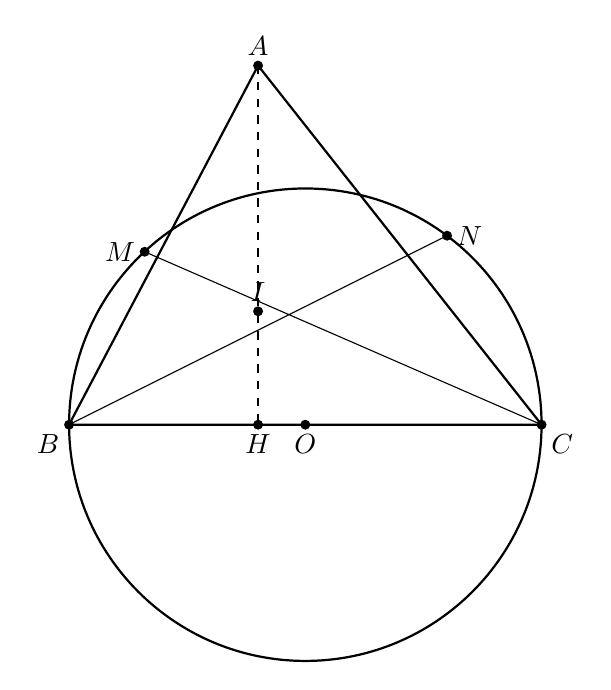
\begin{tikzpicture}[>=stealth, scale=1.2]
		\coordinate (O) at (0,0);
		\coordinate (B) at (-2.5,0);
		\coordinate (C) at (2.5,0);
		\draw[thick] (O) circle (2.5);
		\coordinate (A) at (-0.5,3.8);
		\coordinate (M) at (-1.7,1.83);
		\coordinate (N) at (1.5,2);
		\coordinate (I) at (-0.5,1.2);
		\coordinate (H) at (-0.5,0);
		\draw[thick] (A) -- (B) -- (C) -- cycle;
		\draw (B) -- (N) (C) -- (M);
		\draw[thick, dashed] (A) -- (H);
		\fill (O) circle (1.5pt) node[below] {$O$};
		\fill (B) circle (1.5pt) node[below left] {$B$};
		\fill (C) circle (1.5pt) node[below right] {$C$};
		\fill (A) circle (1.5pt) node[above] {$A$};
		\fill (M) circle (1.5pt) node[left] {$M$};
		\fill (N) circle (1.5pt) node[right] {$N$};
		\fill (I) circle (1.5pt) node[above] {$I$};
		\fill (H) circle (1.5pt) node[below] {$H$};
	\end{tikzpicture}
\end{center}
\begin{enumerate}[a)]
	\item Vì $M, N$ thuộc đường tròn đường kính $BC$ nên:
	$$\widehat{BMC} = 90^\circ \implies CM \perp AB;\quad \widehat{BNC} = 90^\circ \implies BN \perp AC.$$
	Trong tam giác $ABC$, hai đường cao $BN$ và $CM$ cắt nhau tại $I$, do đó $I$ là trực tâm của tam giác $ABC$.\\
	Suy ra $AI$ là đường cao thứ ba, do đó $AI \perp BC$.\\
	Xét tứ giác $MANI$ có:
	$$\widehat{AMI} = 90^\circ\text{ (do } CM \perp AB\text{)},\quad \widehat{ANI} = 90^\circ\text{ (do } BN \perp AC\text{)}.$$
	Suy ra $\widehat{AMI} + \widehat{ANI} = 90^\circ + 90^\circ = 180^\circ$.\\
	Vậy $MANI$ là tứ giác nội tiếp đường tròn đường kính $AI$.
	\item Vì $D$ là điểm chính giữa của cung nhỏ $MN$ nên hai cung bằng nhau: cung $DM = \text{cung } DN$.\\
	Suy ra $\widehat{DBM} = \widehat{DCN}$ (hai góc nội tiếp cùng chắn hai cung bằng nhau).\\
	Xét $\triangle PBM$ và $\triangle QCN$ có:
	$$\widehat{PMB} = \widehat{QNC} = 90^\circ,\quad \widehat{PBM} = \widehat{QCN}.$$
	Suy ra $\triangle PBM \sim \triangle QCN$ (g.g) $\implies \widehat{BPM} = \widehat{CQN}$.\\
	Mặt khác, $\widehat{DPC} = \widehat{BPM}$ (đối đỉnh) và $\widehat{DQB} = \widehat{CQN}$ (đối đỉnh).\\
	Suy ra $\widehat{DPC} = \widehat{DQB}$.\\
	Xét $\triangle DPC$ và $\triangle DQB$ có:
	$$\widehat{BDC}\text{ là góc chung},\quad \widehat{DPC} = \widehat{DQB}.$$
	Suy ra $\triangle DPC \sim \triangle DQB$ (g.g).\\
	Từ đó ta có tỉ số đồng dạng:
	$$\dfrac{DP}{DQ} = \dfrac{DC}{DB} \implies DQ \cdot CD = BD \cdot DP.$$
	Vì $\widehat{IPD}$ kề bù với $\widehat{DPC}$ và $\widehat{IQD}$ kề bù với $\widehat{DQB}$, mà $\widehat{DPC} = \widehat{DQB}$ nên suy ra:
	$$\widehat{IPD} = \widehat{IQD}.$$
	\item Xét $\triangle AMN$ và $\triangle ACB$ có:
	$$\widehat{BAC}\text{ là góc chung},\quad \widehat{AMN} = \widehat{ACB}\text{ (cùng bù với }\widehat{BMN}\text{ do tứ giác } BMNC \text{ nội tiếp)}.$$
	Suy ra $\triangle AMN \sim \triangle ACB$ (g.g).\\
	Do đó $\dfrac{MN}{BC} = \dfrac{AM}{AC}$.\\
	Trong tam giác $AMC$ vuông tại $M$, ta có:
	$$\dfrac{AM}{AC} = \cos \widehat{BAC} = \cos 60^\circ = \dfrac{1}{2}.$$
	Suy ra:
	$$MN = \dfrac{1}{2} BC = \dfrac{1}{2} \cdot 10 = 5\text{ (cm)}.$$
	Vì tứ giác $MANI$ nội tiếp đường tròn đường kính $AI$ nên đường tròn ngoại tiếp tam giác $MIN$ chính là đường tròn đường kính $AI$.\\
	Xét $\triangle AMI$ và $\triangle CMB$ có:
	$$\widehat{AMI} = \widehat{CMB} = 90^\circ,\quad \widehat{MAI} = \widehat{MCB}\text{ (cùng phụ với }\widehat{ABC}\text{)}.$$
	Suy ra $\triangle AMI \sim \triangle CMB$ (g.g) $\implies \dfrac{AI}{BC} = \dfrac{AM}{CM}$.\\
	Trong tam giác $AMC$ vuông tại $M$, ta có:
	$$\dfrac{AM}{CM} = \cot \widehat{BAC} = \cot 60^\circ = \dfrac{\sqrt{3}}{3}.$$
	Suy ra:
	$$AI = BC \cdot \dfrac{\sqrt{3}}{3} = 10 \cdot \dfrac{\sqrt{3}}{3} = \dfrac{10\sqrt{3}}{3}\text{ (cm)}.$$
	Chu vi đường tròn ngoại tiếp tam giác $MIN$ là:
	$$C = \pi \cdot AI = \dfrac{10\sqrt{3}\pi}{3}\text{ (cm)}.$$
\end{enumerate}
}
\end{bt}
